% ============================================
% SECTION 1: Introduction
% ============================================
\section{Introdução}

\begin{frame}{Contexto - Documentos e Compliance}
\begin{itemize}
    \item Documentos físicos
    \item Imagens de documentos
    \item Exemplos:
    % \begin{itemize}
    %     \item Carteira de identidade
    %     \item Carteira de habilitação
    %     \item Recibos
    %     \item Contratos
    % \end{itemize}
    \begin{center}
    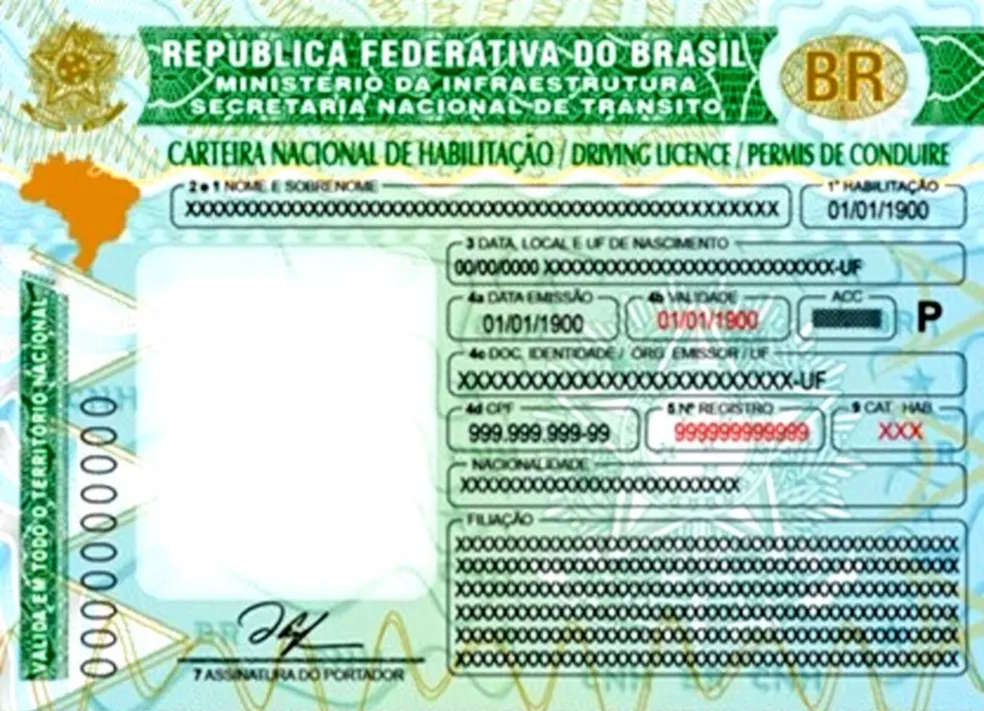
\includegraphics[width=0.27\textwidth]{images-apresentacao/CNH_EXEMPLO.jpg}
    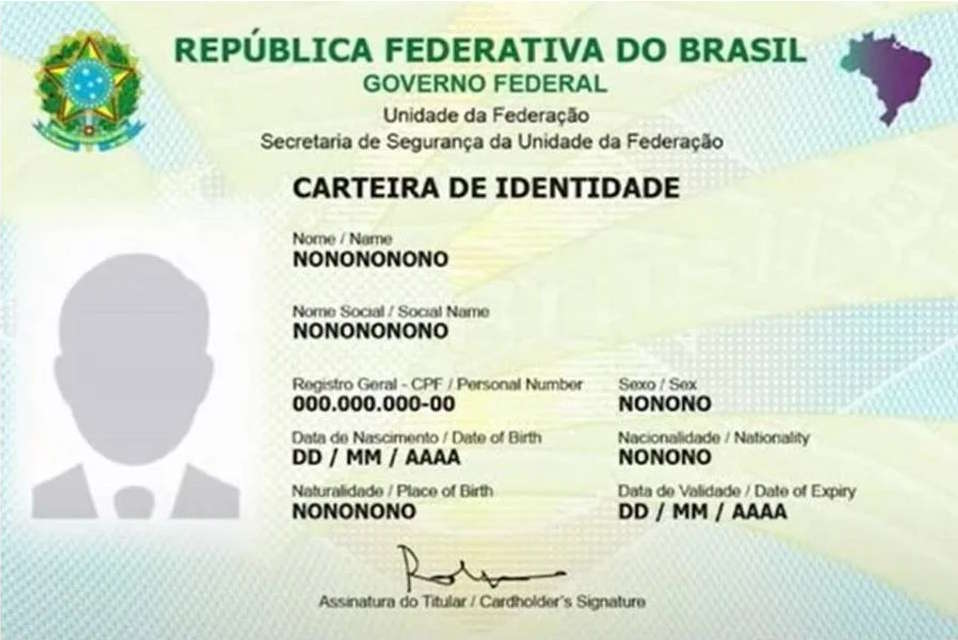
\includegraphics[width=0.29\textwidth]{images-apresentacao/CIN_EXEMPLO.jpg}
    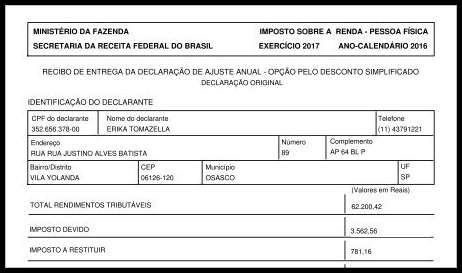
\includegraphics[width=0.33\textwidth]{images-apresentacao/IRPF_EXEMPLO.jpg}
\end{center}
\end{itemize}
\end{frame}


\begin{frame}{Contexto - Processamento de Documentos}
\begin{center}
% Sobreposição de imagens usando tikz
\begin{tikzpicture}
    % Imagem de fundo (diagrama)
    \node[anchor=center] at (0,0) {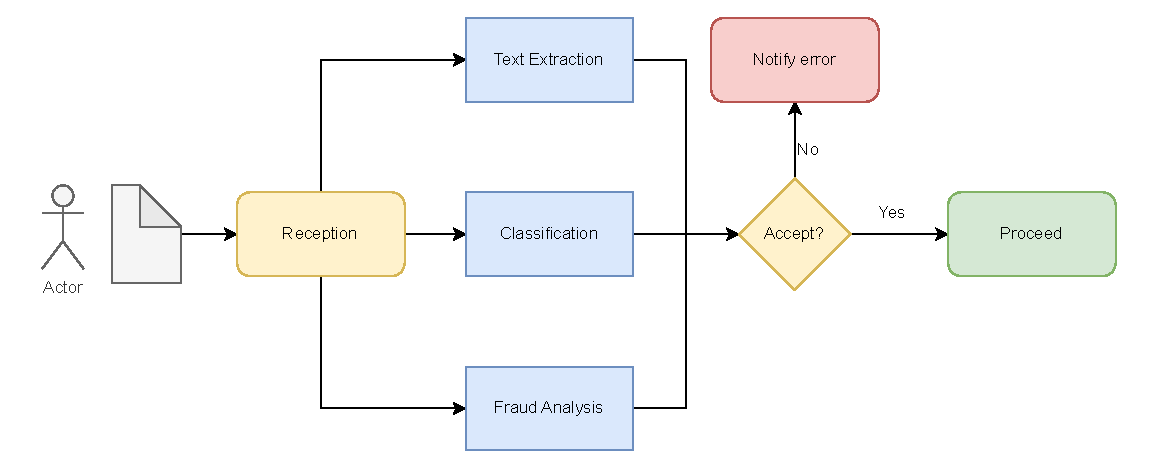
\includegraphics[width=1\textwidth]{images/diagrama-compliance.drawio.pdf}};
    
    % Imagem sobreposta (documento) - ajuste a posição (x,y) conforme necessário
    \node[anchor=center] at (-6,2.5) {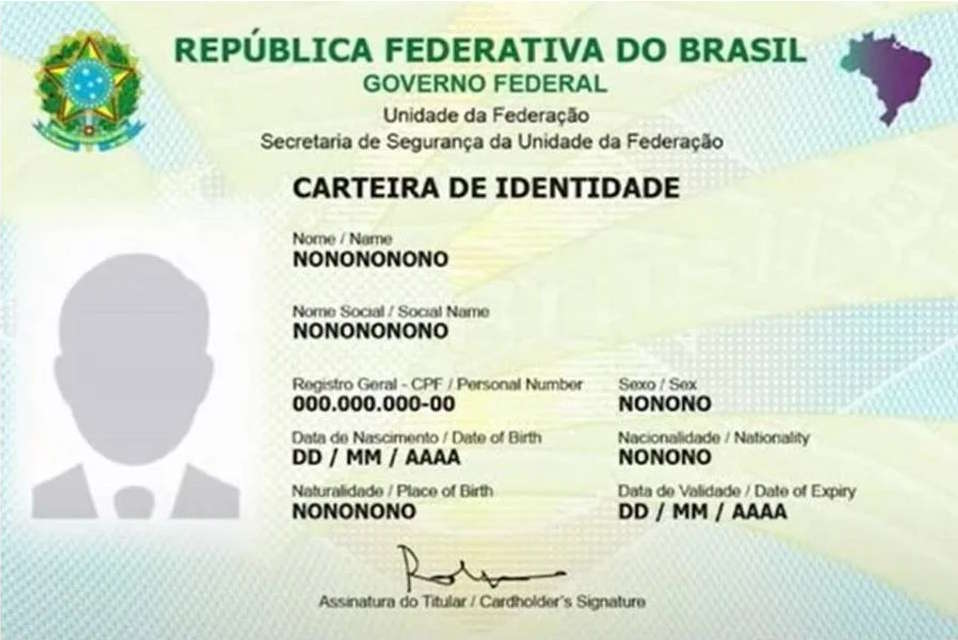
\includegraphics[width=0.18\textwidth]{images-apresentacao/CIN_EXEMPLO.jpg}};
\end{tikzpicture}
\end{center}
\end{frame}

\begin{frame}{Contexto - Importância da Classificação da Imagem}
\begin{columns}
\column{0.5\textwidth}
\begin{itemize}
    \item Assegurar que o documento está correto
    \item Documentos não-digitais
    \item Evita fraudes
\end{itemize}

\column{0.5\textwidth}
\pause
\begin{center}
    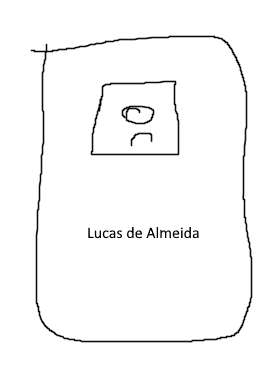
\includegraphics[width=.6\textwidth]{images-apresentacao/EXEMPLO_FRAUDE_CIN.jpg}
\end{center}
\end{columns}
\end{frame}


\begin{frame}{Contexto - Importância da Classificação}
\begin{columns}
\column{0.5\textwidth}
\textbf{Classificação Tradicional:}
\begin{itemize}
    \item Categorização em classes predefinidas
    \item Cross-Entropy Loss
\end{itemize}

\textbf{Desempenho Atual:}
\begin{itemize}
    \item Bakkali et al. (2021): 97.70\% de acurácia no RVL-CDIP
\end{itemize}

\column{0.5\textwidth}
\pause
\textbf{O Problema:}
\begin{itemize}
    \item Novos layouts de documentos
    \item Classes completamente novas
    \item Necessidade de retreinamento
    \item Semanas/meses de engenharia de dados e treinamento
\end{itemize}

% \textbf{Solução:}
% \begin{itemize}
%     \item Técnicas de Zero-Shot Learning (ZSL)
%     \item Generalização para classes não vistas
% \end{itemize}
\end{columns}
\end{frame}

\begin{frame}{Solução}
    \begin{center}
        {\Huge \textbf{Zero-Shot Learning}}\\ \vspace{0.5cm}
        Permite que o modelo reconheça elementos de\\ classes nunca vistas no treinamento
    \end{center}
\end{frame}

\begin{frame}{Sobre a Pesquisa}
\begin{block}{Desafios}
    
    \begin{itemize}
        \item {\large Falta de dataset especializado}
        \begin{itemize}
            \item Imagens de Documento
            \item Generalização
            \item Divisão treino e teste zero-shot
        \end{itemize}
        \item {\large Ausência de metodologia estado-da-arte}
        \begin{itemize}
            \item Paradigma ZSL
            \item Capacidade de classificar
        \end{itemize}
    \end{itemize}
    
\end{block}
\end{frame}

\begin{frame}{Sobre a Pesquisa}
\begin{block}{Contribuições}
    \begin{enumerate}
        \item \textbf{Novo dataset LA-CDIP}
        \begin{itemize}
            \item Classificação ZSL
            \item Derivado do RVL-CDIP
        \end{itemize}
        
        \item \textbf{Abordagem de Visual Document Matching (VDM)}
        \begin{itemize}
            \item Similaridade de documentos
            \item Metric Learning
            \item Generalização Zero-Shot
        \end{itemize}
        
        \item \textbf{Avaliação sistemática}
        \begin{itemize}
            \item Benchmark extensivo
            \item Comparação com LLM
        \end{itemize}
    \end{enumerate}
\end{block}
\end{frame}
